\documentclass[letterpaper,12pt]{article}

% ============================================================
% LaTeX PREAMBLE
% ============================================================

% ---------- CHOOSE A FONT ----------

\usepackage{palatino,mathpazo}             % Palatino
\RequirePackage[scaled=0.92]{helvet}
\RequirePackage[scaled=1.02]{inconsolata}
\linespread{1.05}
\usepackage[T1]{fontenc}

% --------- MISC FORMATTING ---------
%
\usepackage{setspace}                % needed for doublespacing
\doublespacing                       % doublespaced line spacing
\usepackage{natbib}                  % for our chosen bibliography style
\usepackage{graphicx}                % for importing graphics into figures
\usepackage{float}                   % better control of figure placement
\usepackage[margin=1.0in]{geometry}  %	 control page margins
\usepackage[short]{datetime}         % precise date/time stamp on titlepage
\usepackage[labelfont=bf]{caption}   % make caption labels boldface

\usepackage{authblk}                 % author and affiliation formatting
\renewcommand\Affilfont{\small}      %
\setlength{\skip\footins}{10mm}      % obsessing about footnote spacing
\setlength{\parskip}{1ex}            % space between paragraphs
\usepackage{lineno}                  % add line numbers to margin
\linenumbers
\usepackage{authblk}                 % author and affiliation formatting%
\usepackage{lipsum}   

% ------- CUSTOM TITLE FORMAT -------

\makeatletter
\renewcommand{\maketitle}{
\begin{flushleft}       % right align
{\LARGE\@title}         % increase the font size of the title
\vspace{20pt}\\         % vertical space between the title and author name
{\large\@author}        % author name
\\\@date                % date
\vspace{20pt}           % vertical space between the author block and abstract
\end{flushleft}
}

% ============================================================
% TITLE & AUTHORS & AFFILIATIONS
% ============================================================

% Add authors and affiliations as required
\title{This is the title of the manuscript}
\author[1,2,*]{Martin H\'{e}roux}
\author[1,2,3]{Ford Prefect}
\affil[1]{Neuroscience Research Australia}
\affil[2]{School of Medical Sciences, University of New South Wales}
\affil[3]{Hitchhikers guide to the galaxy}
\date{}

% ============================================================
% START OF DOCUMENT
% ============================================================

\begin{document}

% ============================================================
% TITLE PAGE
% ============================================================

% Make title and style changes (don't touch)
\begin{singlespace}
\maketitle
\thispagestyle{empty}
\hfill
\begin{flushleft}

% Set name and mailing address of corresponding author
\vspace{35mm}
$^{*}$\textbf{Corresponding Author}\\
\vspace{2ex}
Martin H\'{e}roux, PhD\\
Neuroscience Research Australia\\
Margarete Ainsworth Bldg, Barker Street\\
Randwick, NSW, Australia 2031	\\
Phone: +612 9399 1842\\
Fax: +612 9399 1005\\
email: m.heroux@neura.edu.au

% ============================================================
% KEYWORDS
% ============================================================

% Set keywords (replace blah; blah)
\vfill
\textbf{Keywords}: blah; blah\\
\vspace{3ex}
\footnotesize{\emph{\today, \currenttime}}
\end{flushleft}
\end{singlespace}

% ============================================================
% ABSTRACT
% ============================================================

\newpage
\section*{Abstract}
This is a cool area of research and others have studied it. 
The purpose of this study was to determine whether Ernie and Bert were a couple.
\lipsum[1]

% ============================================================
% INTRODUCTION
% ============================================================

\newpage
\section*{Introduction}

Lots of crazy research has been done on this topic \citep{Heroux:2015}. 
Even more stuff will be done later. 
But for now I want to focus on the present research questions \citep{Butler2003}.

There was a good point made by a Canadian \citep{Brownstone2006}. 
In fact, \cite{Sawczuk1995} even agreed despite being an American.

\lipsum[1]

% ============================================================
% METHODS
% ============================================================

\section*{Methods}

This is were I would write about the subjects that were recruited for the study. 
I would also state that I have received ethical approval for the study.

\subsection*{Experimental set-up}

This is were I would describe the equipment,the position of the subject and any other relevant things related to the experimental set-up.

\subsection*{Experimental procedures}

This is where I would describe how the study was conducted. 
The various trials, the durations, the order, and any other details of the how the experiment were carried out should be included here.

This section may have more than one paragraph to describe the various portion of the protocol.

\subsection*{Data analysis}

This section will describe how the various measures and signals were processed (e.g., filtered). 

\subsection*{Statistical analysis}

This section will describe the various statistical analyses that were carried out on the data.

% ============================================================
% RESULTS
% ============================================================

\section*{Results}

If you look at Table~\ref{tbl:somedata}, the numbers are totally meaningless. 
But the start-end values were very informative (Table~\ref{tbl:someOtherData}). 
The same goes for Figure~\ref{fig:rawMU}.

\lipsum[1]

% ============================================================
% DISCUSSION
% ============================================================

\section*{Discussion}

As you can see, we were the first to show these results and they will be so very helpful to the world, and possibly even the universe.

\lipsum[1-3]

% ============================================================
% ACKNOWLEDGEMENTS
% ============================================================

\newpage
\section*{Acknowledgements}

This research was supported by an NMHRC Program Grant.

% ============================================================
% REFERENCES	
% ============================================================

\newpage
\bibliographystyle{./refs/jneurophysiol}
\bibliography{./refs/ref_list}

% ============================================================
% TABLES
% ============================================================

% Table 1.
\newpage
\clearpage
\parbox[c][\textheight][s]{\linewidth}{%
\begin{table}[H]
	\centering
	\begin{tabular}{c|c}
		condition &mean\\
		\hline\hline
		A         &10.1\\
		B         &11.0\\
	\end{tabular}
 \caption{Blah blah some data.}
 \label{tbl:somedata}
\end{table}
}

% Table 2.
\newpage
\clearpage
\parbox[c][\textheight][s]{\linewidth}{%
\begin{table}[H]
	\centering
	\begin{tabular}{c|c}
		start &end\\
		\hline\hline
		1.23         &4.5\\
		2.3         &3.90\\
	\end{tabular}
 \caption{Import values.}
 \label{tbl:someOtherData}
\end{table}
}
 
% ============================================================
% FIGURES
% ============================================================

\newpage
\clearpage
\parbox[c][\textheight][s]{\linewidth}{%
\begin{figure}[H]
	\centering
    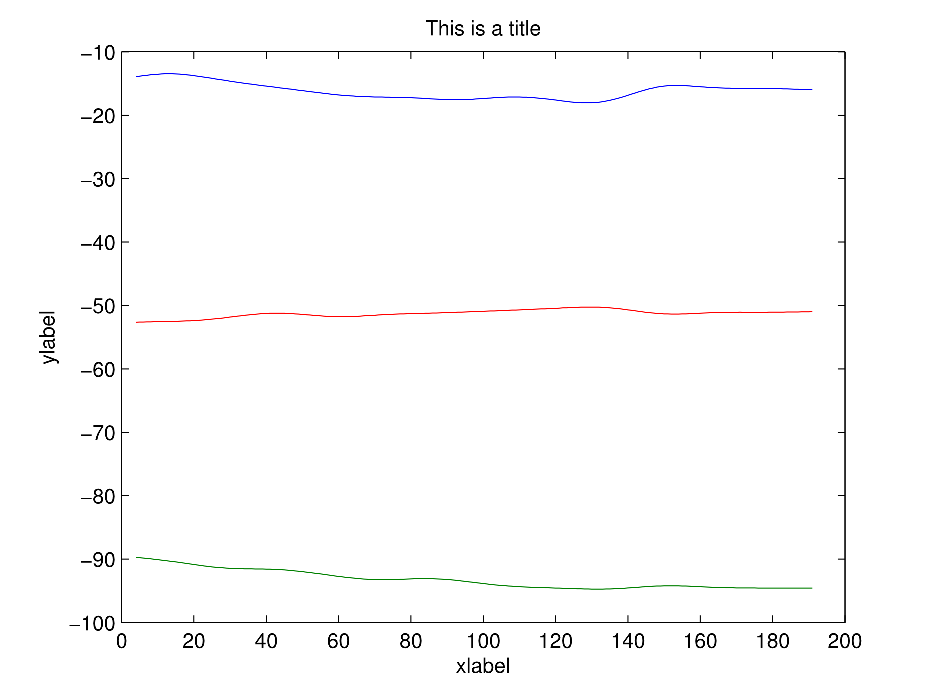
\includegraphics{./figures/fig1.pdf}
 \caption{Blah blah blah.}
 \label{fig:rawMU}
\end{figure}
}

\end{document}